\chapter{Theoretical background}

\section{Need for new technologies to reduce reliance on fossil-based resources} 
% Lisaksin teoreetilise osa esimeseks peatükiks üldise kirjelduse vajadusest vähendada fossiilsete materjalide osakaalu ning selle mitigeerimiseks 
% on ühe võimalusena võimalik kasutada biotehnoloogilisi protsesse, mis suudavad konverteerida jääk-biomassi erinevateks kemikaalideks ning materjalideks. 
% Siit saaks siis otse edasi liikuda R. toroloidese kirjeldusele, kui ühele potentsiaalsele rakuvabrikule biotehnoloogiliste protsesside läbiviimisel. % Petri soovitus

% Due to the massive increase in the utilization of petroleum, it has 
% been predicted that the world will run short of petroleum by the year 
% 2070 \cite{ShieldsMenard2018}. 

% Besides, its widespread usage has also brought global warming 
% and health concerns due to the release of greenhouse and toxic gases 
% such as carbon monoxide, carbon dioxide, methane, and chlorofluorocarbons. Therefore, alternative energy sources that are easily accessible, 
% greener, and readily available are highly required. Due to properties 
% such as non-toxic, biodegradability, being sulfur-free, and the ability of 
% production from renewable sources, biofuels have gained the interest as 
% an alternative to petroleum. \cite{Saini2020}

Many countries globally are developing a bio-based economy to fight climate change and to lower the
reliance on fossil-based resources \cite{Zuiderveen2023}. In Europe, 
the Bio-Economy Strategy was developed to steer Europe towards a sustainable 
bio-based economy and it was reinforced in the European Green Deal aiming for 
climate neutrality by 2050 \cite{Research2018}. Bio-based products may enhance environmental 
sustainability compared to fossil based equivalents \cite{Zuiderveen2023}.

The shift towards a bioeconomy needs novel processes for production of chemicals, materials, 
and liquid fuels from sustainable substrates, that offer improved life cycle 
assessments, and use less energy to produce. Recent advancements have highlighted the 
potential of chemicals derived from plant oils and animal fats as alternative 
feedstocks to the petrochemical industry. 

These feedstocks comprise a broad spectrum of molecules that can be utilized in 
various applications such as biofuels, cosmetics, plastics, 
surface coatings, surfactants, lubricants, paints, etc. \cite{Lopes2020}. Biodiesel is synthesized through the transesterification of triacylglycerols with short-chain alcohols 
(primarily methanol or ethanol) to yield monoalkyl esters, specifically fatty acid methyl esters (FAMEs) 
and fatty acid ethyl esters (FAEEs) \cite{Koutinas2014}.

The growth of worldwide biodiesel production drives the need to increase the 
production of fatty acid methyl esters \cite{Yang2018}. But the production of biodiesel from oilseeds and waste oils doen not sustain the 
global demand \cite{Koutinas2014} and the recent food crisis has shown the 
need for the development of second-generation biofuels derived from 
lignocellulosic raw materials and industrial waste streams \cite{Koutinas2011}.

Microbial lipids are another source of fatty 
acids considered as a potential feedstock for oleochemical production \cite{Unrean2017}. Research has focused on the development 
of biodiesel production from single cell 
oil (SCO) that are produced via fermentation using oleaginous microorganisms (microorganisms 
capable of accumulating lipids at more than 20\% of the total cellular dry weight). 
 
Biodiesel production from SCO relies on the utilization of low-value waste streams 
or residues, thus presenting a sustainable alternative for biofuel production. 
Moreover, the production of SCOs does not require land or other resources that are typically used for food production 
and it is not influenced by season or climate. \cite{Koutinas2014} 


\section{\textit{Rhodotorula toruloides}} % {Physiological characteristics} % General Physiological characteristics {Central carbon metabolism}

\textit{Rhodotorula toruloides} (previously \textit{Rhodosporidium toruloides}) is an oleaginous yeast
which can accumulate lipids up to 76.1\% of cell dry weight \cite{Li2007}. 
What is more, \textit{R. toruloides} has good tolerance to inhibitory compounds that are naturally found in biomass hydrolysates \cite{Hu2009}.
It is one of the most promising yeasts for 
sustainable production of chemicals and fuels \cite{Rekena2023}.

The majority of the lipids produced by \textit{Rhodotorula toruloides} are
triacylglycerol (TAG) contained long-chain fatty acids (C16:0 
(palmitic acid), C16:1 (palmitoleic acid), C18:0 (stearic acid), C18:1(oleic acid), and C18:2 (linoleic acid)) and they
are comparable to vegetable oils \cite{Li2007}, \cite{Vasconcelos2019}.

\textit{R. toruloides} occurs naturally in leaves, soil, sea water, etc. It has a broad substrate range, 
which has made this yeast a popular for producing biological oils from inedible 
substrates such as pentose sugars and crude glycerol. \cite{Tiukova2019} 
\textit{R. toruloides} lipid fraction contains also carotenoid pigments, 
omega-3 linolenic acid and heptadecenoic acid,
which makes it a promising organism for production of pharma- and nutraceuticals \cite{Buzzini2007}. 

One of the major determinants of the oleaginous phenotype of \textit{R. toruloides} is its capacity for acetyl-coenzyme A (acetyl-CoA) production. 
\textit{R. toruloides} possesses the enzyme ATP-citrate lyase (ACL), 
which has been suggested to be the main source of acetyl-CoA for lipid
synthesis in oleaginous species, as it has not been found to be present in non-oleaginous yeasts \cite{Vorapreeda2012}. Mitochondrial beta-oxidation pathway
provides additional source of acetyl-CoA in \textit{R. toruloides}. \cite{Tiukova2019}
Synthesis of acetyl-CoA from xylulose 5-phosphate by phosphoketolase (XPK), and the conversion of S-malate into pyruvate by 
malic enzyme (ME) that provides for nicotinamide adenine dinucleotide phosphate (NADPH) enzymatic pathways, also differ from the model yeast \textit{Saccharomyces
cerevisiae} and which specifically facilitate the generation of lipid precursors.\cite{Rekena2023}
Lipid biosynthetic reactions downstream of acetyl-CoA synthesis do not differ between oleaginous and non-oleaginous 
yeast species \cite{Tiukova2019}.

In \textit{R. toruloides} metabolic pathways producing acetyl-CoA and a cofactor NADPH
have been the main focus of metabolic studies due to their central role in lipid
biosynthesis. Fatty acids mainly accumulate as TAGs, and they are
produced via four enzymatic reactions that require 1 ATP and 2 NADPH molecules for adding 1 acetyl-CoA to the fatty acid chain \cite{Lian2015}.
Proteomics analysis has suggested that NADPH is primarily regenerated through the pentose phosphate pathway, when grown on xylose 
and glucose, but the role of malic enzyme is not clearly understood. The
role of XPK in the generation of acetyl-CoA has not been acknowledged previously, whereas
ACL has been demonstrated to be upregulated during lipid accumulation, especially in
presence of xylose.\cite{Rekena2023} 



\section{Overview of cellular growth laws}

Lipid accumulation in oleaginous microorganisms has long been known to be triggered 
by a nutrient imbalance in the culture medium. When cells run out of a key nutrient, 
usually nitrogen, excess carbon substrate continues to be assimilated by the cells 
and converted into storage fat. Cells assimilate carbon quicker than they can convert 
it into new cells so mechanism for storage the excess carbon is then found by 
converting it into lipid. Lipid accumulation requires a slow growth rate of the cells 
to allow the excess carbon to be assimilated faster than it can be converted into 
biomass so that the surplus carbon is channeled into lipid. 
With oleaginous yeast the process of lipid accumulation can also 
be achieved in continuous culture, where is it necessary to grow the 
cells at a sufficiently low dilution rate (= growth rate) to allow the cells to 
assimilate the glucose. The results from continuous cultivation studies clearly 
indicate that the rate of lipid synthesis is slower than the maximum growth rate. \cite{Ratledge2002}

Lipid accumulation occurs when oleaginous microorganisms are cultivated in a medium with an excess of 
carbon where other nutrients, particularly nitrogen, is limiting their growth. 
Therefore, the carbon-to-nitrogen ratio (C/N) plays an important role in triggering
lipid accumulation. \cite{Lopes2020}

What is the biochemical difference between these two groups of very distinct microorganisms? 
The first major biochemical difference to be identified between the oleaginous and nonoleaginous 
yeast species was the presence of ATP-citrate lyase in oleaginous yeast during lipid accumulation.
ACL has proved to be one of the key enzymes that must be present in a eukaryotic microbial 
cell for it to be able to accumulate substantial amounts of triacylglycerol lipids.
In those yeasts without ACL, lipid contents of the cell were invariably low. However, 
some yeasts had ACL activity but did not accumulate lipid,  thus indicating that 
other enzyme activities were needed to ensure lipid accumulation. In summary, while 
the possession of ACL activity will not automatically engender lipid accumulation 
in a microorganism, if the enzyme is absent the cells will be unable to accumulate 
lipid and will therefore be nonoleaginous. Clearly, other enzyme activities must be 
in place to determine the extent to which lipids may accumulate in individual 
organisms. \cite{Ratledge2002}

Malic enzyme has found to be another important enzyme in lipogenesis. It generates 
NADPH, which is used by fatty acid synthetase (NADPH is generated also by 
glucose-6-phosphate dehydrogenase, 6-phosphogluconate dehydrogenase, and NADP-dependent 
isocitrate dehydrogenase). When malic enzymes activity was blocked by using selective inhibitors (sesamol), 
he content of lipid in the cells was decreased by almost 90\%, from 24\% 
of the cell biomass to 2\% but — and this was of major significance — without causing 
any major effect on growth. Thus, as only malic enzyme activity appeared to have been affected 
by the inhibitor, it was concluded that 
sesamol was specifically inhibiting both the cytoplamic and membrane-bound malic 
enzymes, and that without malic enzyme the cell was unable to accumulate lipid or 
to carry out desaturations of it. The essentiality of malic enzyme for lipid 
biosynthesis appeared to be established.
\cite{Ratledge2002}

Wynn and Ratledge (1997) went on to show that in a mutant of \textit{Aspergillus Nidulans} lacking 
malic enzyme activity, only half the lipid (12\% of the cell dry weight) that had been 
produced by the competent strain under nitrogen-limited growth conditions was now 
produced. \cite{Ratledge2002}
Fatty acid biosynthesis per se is still functional and phospholipids can be produced. 
Thus, the cell can manage without malic enzyme—it is not absolutely vital—but the cell
cannot produce storage triacylglycerols in any abundance. Without malic enzyme 
activity the flux of carbon, from glucose to lipid, is considerably diminished and 
only essential lipids are produced—presumably by using other sources of NADPH. \cite{Ratledge2002}




\section{Overview of microbial cultivation methods}


\section{Genome-scale metabolic modeling} %incl. Constraint-based modeling, kinetic modeling, steady-state, limitations, e.g. regulation

Genome-scale metabolic models (GEMs) are comprehensive descriptions of all known metabolic reactions of a
organism, which are derived from the organism's available genome sequence \cite{Kerkhoven2014}. 
GEMs account for genes, proteins, and biochemical reactions, which enable systematic
analysis of metabolism, where typically the objective is to achieve a global picture of possible flux
patterns \cite{Kerkhoven2014}\cite{Chen2023}. 

A microorganism's phenotype can be described by its pattern of metabolic fluxes \cite{Kerkhoven2014}. 
Metabolic flux is the rate of turnover of molecules through a metabolic pathway. Flux is regulated by the enzymes involved in this pathway. Within cells, 
regulation of flux is vital for all metabolic pathways to regulate the pathway's activity under different conditions. \cite{Voet1995} In biotechnology the aim is often 
to increase the capacity of specific fluxes. For this, metabolic engineering methods have been developed and many of these 
rely on balancing intracellular metabolites using GEMs that in
combination with appropriate objective functions and constraints can be used to predict potential gene 
targets for obtaining a preferred flux distribution. \cite{Kerkhoven2014} 

GEMs can be a powerful and helpful tool in metabolic studies, if their predictive 
power is good \cite{Rekena2023}. The use of GEMs enables the integration of omics data and experimental metabolic fluxes to generate a holistic 
view of metabolism in different physiological states, allowing a greater understanding of cellular physiology and providing valuable information 
for metabolic engineering and the development of microbial factories as a whole. \cite{DeBiaggi2023} The number of organisms for which metabolic 
reconstructions have been created is increasing at a pace similar to whole genome sequencing. \cite{Thiele2010}

The metabolic reconstruction process usually is very labor- and time consuming. For for well-studied, medium genome sized bacteria it can take around six months to reconstruct the model. The  
metabolic reconstruction of human metabolism can take up to two years and six people. The reconstruction process is often iterative, for example the reconstruction of metabolic 
network of \textit{Escherichia coli} has been expanded and refined throughout the last 19 years. Despite growing experience and 
knowledge, it is still not possible to completely automatically reconstruct high-quality metabolic networks which can be used as reliable predictive models. \cite{Thiele2010} 
(See appendix A for more detailed reconstruction process.) 


\textbf{Constraint-based modeling}

Genome-scale metabolic models are widely used to calculate metabolic phenotypes, but as metabolism operates under countless of constraints, they rely on defining a set of constraints. 
They include constraints that 
remain unchanged as they come by the laws of physics (e.g. conservation of mass and energy, thermodynamics), 
and constraints that can vary by organism, environmental condition, the state of the 
cell (e.g. nutrient uptake rate, biomass composition), and constraints that can also change through evolution or 
changes in gene expression. \cite{Kerkhoven2022}

A major limitation in the predictive power of conventional GEMs is that enzyme abundances and kinetics, which act as limitations on 
metabolic fluxes, are not taken into account. When considering the production of a metabolite of interest, 
these models typically make the assumption that the uptake rate of the carbon source limits production. 
This may be an oversimplification, as metabolic fluxes are limited by their corresponding enzyme levels. \cite{Sanchez2017}
The synthesis of enzymes is resource- and energy-expensive, their catalytic 
capacities are limited by their kinetics, what is more, the quantity of enzymes is space-constraint \cite{Kerkhoven2022}.

This means that an increase in the requirement of an enzyme or a pathway would be a trade-off for other
functions. Experimental evidence indicates that for various organisms resource re-allocation could be an effective strategy 
in response to nutrient and growth shift, which demonstrates the biological significance 
of proteome constraints. \cite{Chen2023} 
Applying such constraints in a metabolism model reduces simulated flux distributions to those that are most 
economic and also limits the phenotypes that the model can simulate. These both contribute to more realistic results. 
Such models have already found numerous applications in e.g. unraveling the underlying mechanisms for observed metabolic 
phenotypes and the prediction of strain optimization strategies. \cite{Kerkhoven2022}
This suggests that proteome constraints could be a valuable addition to GEMs to
improve model predictions \cite{Chen2023}. 

Integration of enzyme constraints and proteomics data into GEMs was first enabled by the GECKO toolbox, allowing the study of phenotypes constrained by 
protein limitations. GECKO is a method for enhancement of GEMs with Enzymatic Constraints using 
Kinetic and Omics data, developed in 2017. This method extends the classical FBA 
approach by incorporating a detailed description of the enzyme demands for the metabolic reactions in a network, accounting for all types of enzyme-reaction 
relations, including isoenzymes, promiscuous enzymes and enzymatic complexes. Moreover, GECKO enables direct integration of proteomics abundance data, 
if available, as constraints for individual protein demands, represented as enzyme usage pseudo-reactions, whilst all the unmeasured enzymes in the network 
are constrained by a pool of remaining protein mass. \cite{Domenzain2022}

Every metabolic reaction flux has a
biological constraint that is equal to the enzyme's concentration multiplied by its turnover number ($k_{cat}$). Enzyme constraint is
defined as the maximum rate of enzymatic reaction ($v_{max}$) that the metabolic flux cannot exceed. Enzyme-constrained GEMs thereby 
ensure that each metabolic flux does not exceed its biological maximum capacity, 
equal to the product of the enzyme's abundance and turnover number \cite{Sanchez2017}.

Phenomenological constraint is imposed on metabolic flux (v; mmol/gDCW/h), formulated as enzyme
kinetics: $v <=  E \cdot k_{cat}$, where $E$ is protein abundance (mmol/gDCW) and $k_{cat}$ is the enzyme's turnover number (1/s),
provided with an upper limit on individual or total protein abundances. The integration of
enzymatic constraints in \textit{S. cerevisiae} has significantly improved phenotype prediction. \cite{Sanchez2017}

The reconstructed genome-scale networks can be converted into mathematical stoichiometric matrices, where rows represent metabolites 
and columns represent individual reactions. This matrix will
determine the solution space of the metabolic network. GEMs are constrained by (1) the stoichiometry of the
network; (2) preset upper and lower boundaries for selected reactions; and (3) the assumption of a steady state. \cite{Kerkhoven2014} 
Overview of a reconstruction of a GEMs is shown in the figure \ref{GEMs}.


\begin{figure}[h]
    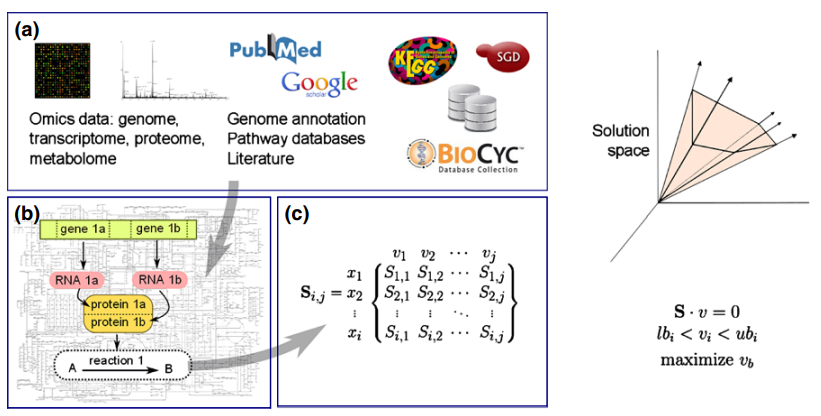
\includegraphics[width=\linewidth]{GEMs.png}
    \caption{Reconstruction of a GEM. (a) The genome annotation is used 
    to reconstruct the draft. (b) Gene-protein-reaction relationships are defined for the metabolic model. 
     (c). A solution space is defined from the constraints applied to the model. Figure is from article \cite{Kerkhoven2014}.}
    \label{GEMs}
\end{figure}




\textbf{Flux balance analysis}

% GEMs can simulate metabolic flux distributions by optimization of an objective function that describes the 
% perceived cellular objective that propels 
% metabolism, by flux balance analysis (FBA). \cite{Kerkhoven2022}
Flux balance analysis (FBA) is a mathematical approach for analyzing the flow of metabolites through a metabolic network.
It is a widely used approach for studying biochemical networks, in particular the genome-scale metabolic network reconstructions. 
FBA calculates the flow of metabolites through this metabolic network, thereby making it possible to predict the growth rate of an 
organism or the rate of production of a biotechnologically important metabolite. 
\cite{Orth2010}

The first step in FBA is to mathematically represent metabolic reactions. 
The core feature of this representation is a tabulation, in the form of a numerical matrix ($S = m\cdot n$), 
of the stoichiometric coefficients of each reaction. These stoichiometries impose 
constraints on the flow of metabolites through the network. Constraints such as these lie at the heart of 
FBA, differentiating the approach from theory-based models based on biophysical equations that require many difficult-to-measure 
kinetic parameters. Every row of this matrix represents one unique compound (for a system with $m$ compounds) and every column 
represents one reaction ($n$ reactions). 

The entries in each column are the stoichiometric coefficients 
of the metabolites participating in a reaction. There is a negative coefficient 
for every metabolite consumed, and a positive coefficient for every metabolite 
that is produced. A stoichiometric coefficient of zero is used for every 
metabolite that does not participate in a particular reaction. $S$ is a sparse 
matrix since most biochemical reactions involve only a few different metabolites. 
The flux through all of the reactions in a network is represented by the vector 
$v$, which has a length of $n$. The concentrations of all metabolites are represented
by the vector $x$, with length $m$. The system of mass balance equations at steady 
state ($dx/dt = 0$) is: $Sv = 0$. \cite{Orth2010}

Steady state assumption presumes that all the flux rates and metabolite concentrations are constant over time. In experiments this state can be
reached in chemostat cultivation and, in theory, during controlled batch logarithmic growth
phase. \cite{Kerkhoven2014} 

Any $v$ that satisfies this equation is said to be in the null space of $S$. In any realistic 
large-scale metabolic model, there are more reactions than there are compounds ($n > m$). In other words, 
there are more unknown variables than equations, so there is no unique solution to this system of equations. \cite{Orth2010}

Although constraints define a range of solutions, it is still possible to identify
and analyze single points within the solution space. For example, we may be 
interested in identifying which point corresponds to the maximum growth rate 
or to maximum ATP production of an organism, given its particular set of 
constraints. FBA is one method for identifying such optimal points within a 
constrained space (see figure below). 

\begin{figure}[h]
    \includegraphics[width=\linewidth]{FBA_solution_space.jpg}
    \caption{Conceptual basis of constraint-based modeling and FBA. The figure is from \cite{Orth2010}.}
    \label{Solution space}
\end{figure}

With no constraints, the flux distribution of a 
biological network may lie at any point in a solution space. When mass balance constraints 
imposed by the stoichiometric matrix $S$ (1) and capacity constraints imposed by the lower and upper 
bounds ($a_i$ and $b_i$) (2) are applied to a network, it defines an allowable solution space. The network 
may acquire any flux distribution within this space, but points outside this space are denied by the 
constraints. 

Through optimization of an objective function, FBA can identify a single optimal flux distribution 
that lies on the edge of the allowable solution space. Optimization of such a system is accomplished by linear 
programming. FBA can thus be defined as the use of linear programming to solve the equation $S\cdot v = 0$ 
given a set of upper and lower bounds on v and a linear combination of fluxes as an objective function. 
The output of FBA is a particular flux distribution, $v$, which maximizes or minimizes the objective function. \cite{Orth2010}

The next step in FBA is to define a biological objective that is relevant to the problem being studied. 
In the case of predicting growth, the objective is biomass production, the rate at which metabolic compounds 
are converted into biomass constituents such as nucleic acids, proteins, and lipids. Mathematically, 
the objective is represented by an objective function that indicates how much each reaction contributes to the phenotype. 
A biomass reaction that drains precursor metabolites from the system at their relative stoichiometries to simulate biomass production is 
selected by the objective function in order to predict growth rates. This reaction is scaled so that the flux through it is equal 
to the exponential growth rate ($\mu$) of the organism.  \cite{Orth2010}

The most commonly used objective function in FBA is maximization of the 
specific growth rate, ATP generation or a certain product formation. FBA is often used for estimating the biotechnological potential of 
microorganisms and pinpoint genetic manipulations that could improve the performance of a cell. The main applications of 
FBA are:\\
(1) Instructions for metabolic engineering purposes; \\
(2) Biological interpretation and discovery through 
contextualizing high-throughput data; \\
(3) Development of a computational framework; \\
(4) Evolutionary elucidation; \\
(5) Description of multispecies communities. \cite{Kerkhoven2014}

Many computational linear programming algorithms exist, and they can very quickly 
identify optimal solutions to large systems of equations. The COBRA Toolbox \cite{Becker2007} is a freely available Matlab 
toolbox for performing these calculations. Models for the COBRA Toolbox are saved in the Systems Biology Markup Language (SBML) \cite{Hucka2003} format.

However, FBA has limitations. Because it does not use kinetic parameters, it cannot 
predict metabolite concentrations. It is also only suitable for determining fluxes 
at steady state. Except in some modified forms, FBA does not account for regulatory effects 
such as activation of enzymes by protein kinases or regulation of gene expression, so its predictions 
may not always be accurate. \cite{Orth2010}

\textbf{Limitations}

GEMs and kinetic models both have their advantages
and drawbacks. GEMs are comprehensive but are dependent on a pseudosteady state and in their current form
do not take regulation, such as gene-protein and protein-protein level interactions, allosteric regulation or 
regulation at post-translational level, into account. At the same time, kinetic models require parameter values that are
difficult to estimate at the global scale. As neither of them can fully replace the other, there has been a considerable
effort on combining these two approaches in a singular model or applying them in succession. \cite{Kerkhoven2014}

GEMs in combination with global datasets are invaluable for detecting
the metabolic bottlenecks, but due to lack of kinetic data about enzyme activities or regulation mechanisms they
are limited in their predictive power. Applying kinetic models on metabolic bottlenecks previously detected with
GEMs can help to understand the regulation or kinetics of these specific enzymatic steps, as one would not need
model parameters for the whole system. \cite{Kerkhoven2014}


\section{Genome-scale metabolic models of \textit{Rhodotorula toruloides}} 
% Tuua välja need erinevad ülegenoomsed mudelid, mis on loodud ning nende peamied iseärasused ja erinevused üksteisest.
% NP11, iRhtoC, IFO0880, IFO0880\_jsb, 

\textbf{rhto-GEM}

The first genome-scale model of \textit{R. toruloides} metabolism named rhto-GEM was presented in 2019 by Tiukova et al. The model includes 4869 genes, 
897 reactions, and 3334 metabolites. The model rhto-GEM, is based on the genome sequence of \textit{R. toruloides} strain 
NP11. To reconstruct those parts of metabolism that are relatively conserved between fungal species, the 
well-curated GEM of Saccharomyces cerevisiae was taken as template model (yeast-GEM version 
8.2.0, 16), while orthologous genes were identified via bi-directional BLASTP against the S. cerevisiae 
S288c reference genome. \cite{Tiukova2019}

To transform this functional draft model to the first version of the \textit{R. toruloides} GEM, additional 
manual curation was performed where remaining template-derived genes were replaced by their \textit{R. toruloides} 
ortholog where possible and otherwise deprecated. Lipid metabolism of \textit{R. toruloides} was described applying 
the SLIMEr formalism as previously described for \textit{S. cerevisiae}, which allows direct 
integration of lipid class and acyl chain experimental distribution data. As the acyl chain distribution of 
\textit{R. toruloides} is different from \textit{S. cerevisiae}, e.g. the presence of C18:2 and C18:3, this required extensive manual curation of the SLIMEr reactions. 
\textit{R. toruloides} specific reactions and pathways, such as carotene and torulene biosynthesis, synthesis 
and degradation of C18:2 and C18:3 fatty acids, and mitochondrial beta-oxidation were subsequently 
manually curated. \cite{Tiukova2019}

The model incorporates knowledge obtained from genomics and proteomics data generated for
\textit{R. toruloides} and was validated using cultivation data. Simulations of rhto-GEM on 
various carbon sources demonstrated good agreement with experimentally reported growth rates. 
Analysis of model allowed to identify potential genetic engineering strategies for enhanced lipid production. 
Some of these genetic targets were found to agree with published experimental studies. 
As such, rhto-GEM emerges as a valuable tool for future analysis of oleaginous and lipid 
metabolism. \cite{Tiukova2019}


\textbf{iRhto1108}

During the same year as rhto-GEM by Tiukova et al. \cite{Tiukova2019} was presented, Dinh et al. \cite{Dinh2019} presented another \textit{R. torluoides} 
genome-scale metabolic model named iRhto1108, collecting and organizing functional genomics data
\cite{Coradetti2018} and prior knowledge. The model is based on the strain IFO0880's metabolic network and it accounts for 2204 reactions, 1985 metabolites and 1108 genes. 

\textit{R. toruloides} has been target of significant research efforts
including genome (re)sequencing, functional genomics analyses, differential omics characterization, determination of macromolecular composition, and growth
kinetics in a continuous culture. These experiments have ushered an improved understanding of \textit{R. toruloides}
metabolism and provided the basis for the reconstruction of a metabolic
model with genome-wide coverage. \cite{Dinh2019}

The authors integrated and supplemented the current knowledge with in-house generated biomass composition and experimental
measurements pertaining to the organism's metabolic capabilities. 
iRhto1108 model integrates yeast biochemistry information from (i) previously built genome-scale
models (\textit{S. cerevisiae} yeast 7.6 \cite{Aung2013}, (ii) KBase fungal
models \cite{Arkin2018}), and (iii) \textit{R. toruloides} specific information
extracted from the primary literature \cite{Coradetti2018}\cite{Jagtap2017}\cite{Kot2018} or generated herein. 
Organism-specific macromolecular composition and ATP maintenance requirements were experimentally measured for two separate growth conditions: (i) carbon and
(ii) nitrogen limitations. Overall, iRhto1108 reproduced \textit{R. toruloides} utilization capabilities for 18 alternate substrates, matched measured wild-type growth yield,
and recapitulated the viability of 772 out of 819 deletion mutants. \cite{Dinh2019}

% Predictions of genotype-phenotype relations were improved through manual curation of 
% gene-protein-reaction rules for 543 reactions leading to correct 
% recapitulations of 84.5\% of gene essentiality data (sensitivity of 94.3\% and specificity of 53.8\%). \cite{Dinh2019}

% An NGAM value of 1.01 mmol gDW-1 hr-1 for both conditions was recovered. In contrast, the growth associated maintenance
% (GAM) was condition-dependent with a value of 140.98 mmol gDW-1
% under carbon limited and 154.94 mmol gDW-1 under nitrogen limited
% conditions. In yeast 7.6, NGAM is not modeled (though an earlier
% S. cerevisiae model (Mo et al., 2009) reported an NGAM value of 1 mmol
% gDW-1) and the GAM value is 59.28 mmol gDW-1. The GAM value
% quantifies growth-associated energy costs that are not captured in the
% biomass equation, alluding to higher energy demands for R. toruloides
% growth compared to S. cerevisiae. \cite{Dinh2019}

% In rhto-GEM model v. 1.1.1 (Tiukova et al., 2019), a non-condition-specific GAM value of
% 132.7 mmol gDW-1 and NGAM value of 3 mmol gDW-1 hr-1 were reported. These values generally match the iRhto1108’s corresponding
% entries under carbon limitation. \cite{Dinh2019}

% Despite careful curation, a large number of blocked reactions (i.e., 677 out of
% 2204) remained in the model spanning multiple pathways. Most of them
% are transport reactions (i.e., 194 reactions) connecting the network. The
% rest participate in secondary metabolism and degradation of amino acids,
% fatty acids, and lipids. We chose to keep them in the hope that they would
% aid in gap-filling attempts in the future.

Essential cellular metabolism and growth
capability of the model were validated extensively with experimental
results, including gene essentiality \cite{Coradetti2018} and growth
data. iRhto1108 was also able to recapitulate experimentally-observed
lipid accumulation phenotypes. iRhto1108 can comprehensively capture \textit{R. toruloides} metabolism and provide meaningful predictions that
were validated with experimental data including suggestion of genetic
perturbations leading to triacylglycerol overproducing strains. Overall, iRhto1108 has undergone a
detailed range of testing and validation studies promising to aid in future
investigations of \textit{R. toruloides}. \cite{Dinh2019}


\textbf{Rt\_IFO0880}

In 2021 Kim et al. performed multi-omics analysis of lignocellulosic carbon utilization in \textit{R. toruloides} and reconstructed
the genome-scale metabolic network named Rt\_IFO0880. The
curated metabolic reconstruction consisted of 1106 genes, 1934
reactions, and 2010 metabolites (1246 unique metabolites) in
nine compartments. \cite{Kim2021}

High-quality metabolic network
models for model organisms and orthologous protein mapping were used to build a
draft metabolic network reconstruction. The reconstruction was manually curated to
build a metabolic model using functional annotation and multi-omics data including
transcriptomics, proteomics, metabolomics, and RB-TDNA sequencing. \cite{Kim2021}

There were many incorrect reactions involved in fatty acid
biosynthesis and beta-oxidation, especially for unsaturated fatty
acids. The reactions and genes in the central metabolic pathways
were manually checked for their co-factor usage and localization. Authors used multi-omics and other experimental measurement
to update the biomass reaction. The DNA composition was
updated using the genome sequence, RNA composition was
updated using transcriptomics data, amino acid composition
was updated using proteomics data, and lipid composition
was updated using fatty acid methyl ester analysis. \cite{Kim2021}
 
Authors performed a genome-scale evaluation and iteratively
improved the model using high-throughput growth phenotyping
and functional genomics. They tested the developed metabolic model's capability to predict
growth on different carbon, nitrogen, sulfur, and phosphate
sources. The model was further refined to resolve the inconsistencies and several genes
with erroneous ortholog mapping were removed from the
model. \cite{Kim2021}

The metabolic network model was validated against high-throughput growth phenotypes in 213 growth conditions and
conditional gene essentiality in 27 growth conditions with high
prediction accuracies, significantly expanding the breadth and
depth of metabolic coverage from previously published models
(\cite{Dinh2019};\cite{Tiukova2019}). \cite{Kim2021}

Authors believe that the
developed metabolic network for \textit{R. toruloides} is most complete
and accurate to date, and the multi-omics data and metabolic
model presented in this study will be useful for studying and
engineering \textit{R. toruloides} for lignocellulosic biomass conversion. \cite{Kim2021}


\textbf{Rt\_IFO0880\_LEBp2023}

 In a doctoral thesis focused on the carotenoid production of \textit{R. torluoides} \cite{DeBiaggi2023} the author compared the four existing GEMs 
 of \textit{R. torluoides} (the ones mentioned before and also rhto-GEM\_BioEng, 
 which is a version of the rtho-GEM with carotenoids integrated into the biomass composition and an alternative xylose assimilation pathway \cite{Pinheiro2020}) and selected the model 
 Rt\_IFO0880 as the best one from the four for further enhancement.

 The author chose the model Rt\_IFO0880, because it was the one
 that needed least improvement and its description of 
 metabolism was the one that best represented the pathways involved in the 
 biosynthesis of carotenoids in \textit{R. toruloides}, according to the study carried out by \cite{DeBiaggi2023}. 
Furthermore, its accuracy and sensitivity are higher than those of the other models, meaning that the Rt\_IFO0880 is more accurate in predicting 
the essentiality of genes compared to the other models. \cite{DeBiaggi2023}

The following changes were made by \cite{DeBiaggi2023}: (i) The reaction and gene-protein-reaction relation (GPR) corresponding to cytosolic malate dehydrogenase (cMDH) were added. The lower and upper 
flow limits of the xylokinase (produces xylulose-5-phosphate) and phytoene dehydrogenase (enzyme in carotenoid byosynthesis) enzymes were equalized to zero to reflect, respectively, 
the absence of detectable activity of the former and the deletion of the gene encoding the latter; 
(iii) A phytoene transport reaction was created for the lipid body compartment to release the flow through the synthesis of this compound; 
(iv) The lower limit of the cytosol-to-phytoene NADP+ transport reaction was changed to a non-zero value (-1000 mmol/gMCS.h) 
to confer reversibility to this reaction. The model updated in this way, called Rt\_IFO0880\_LEBp2023, 
was validated against the experimental data. \cite{DeBiaggi2023}

Unlike its predecessor, GEM Rt\_IFO0880\_LEBp2023 provides for the use of ACL in all maximum theoretical yield of phytoenes scenarios.
This enzyme is extremely abundant in \textit{R. toruloides} 
\cite{Zhu2012} so its prediction by GEMs would be expected. However, from other models only the iRhtoC predicted the use of this enzyme. 
The modification that seems to have allowed the Rt\_IFO0880\_LEBp2023 to predict 
the use of ACL was the addition of cytosolic malate dehydrogenase. This enzyme allows the conversion of oxaloacetate produced by ACL into malate, which in turn is 
transported into the mitochondria into an antiporte with mitochondrial citrate, which is taken to the cytosol to be substrate of ACL. This pathway has recently 
been described as an alternative to the classic 
tricarboxylic acid pathway and has been called the "non-canonical TCA cycle" \cite{Arnold2022}. In addition to the
Rt\_IFO0880\_LEBp2023 model, the iRhtoC model was also able to predict it. The inability of the other models to predict the non-canonical TCA cycle can be explained by the absence of cMDH (Rt\_IFO0880) and citrate-malate antiporte 
between the cytosol and the mitochondria (rhtoGEM and rhtoGEM\_BioEng). \cite{DeBiaggi2023}

The update of the chosen model resulted in the model Rt\_IFO0880\_LEBp2023, presented a better fit to the experimental data
than the others. In addition, this GEM was able to predict the use of the ACL enzyme, an enzyme present in \textit{R. toruloides} according to omics studies \cite{Zhu2012}
but which use was not predicted in three of the four models. 
The prediction of the use of ACL also allowed the observation that \textit{R. toruloides} possibly uses a non-canonical TCA cycle to avoid the production of CO2 in 
the generation of mitochondrial NADH, something previously observed for this yeast. \cite{DeBiaggi2023}

The updated model (Rt\_IFO0880\_LEBp2023) showed a high capacity to adjust to experimental data and to predict the use of biologically relevant enzymes for this yeast, 
such as ACL. Despite the few updates, the best predictions of the Rt\_IFO0880\_LEBp2023 when compared to the other GEMs of \textit{R. toruloides} accredit it as the most faithful
 to the metabolism of this yeast to date. GEM Rt\_IFO0880\_LEBp2023, generated in this work, is the best representative of the metabolism of \textit{R. toruloides}, 
 because it describes more precisely its xylose
 assimilation pathways, the conversion of acetyl-P into acetyl-CoA and the absence of HMG-CoA transport from the mitochondria to the cytosol, 
 (characteristics inherited from its predecessor GEM) and predicts the use of ACL and its involvement in a non-canonical TCA cycle. \cite{DeBiaggi2023}

\textbf{Comparison of the models}

The first model is based on the genome of the NP11 strain, while the other three are based on that of the IFO0880 strain. Both are haploid strains \cite{BANNO1967}; \cite{Zhu2012}. 
The similarity between the genomes of these strains is approximately 95\% \cite{Schultz2022}.

The differences between the models cannot be explained by differences in the genomes of the NP11 and IFO0880 strains, since they exist 
between the iRhtoC and Rt\_IFO0880 models, which are based on the same genome annotation as the latter. In addition, the annotations in 
the genome of \textit{R. toruloides} are still flawed because they are based on genes and metabolic pathways of conventional yeasts. \cite{DeBiaggi2023}

In term of genome coverage, iRhto1108 contains slightly more genes than rhto-GEM (i.e., 1108 vs. 926
genes) or after the removal of blocked reactions (i.e., 806 vs. 624 genes). \cite{Dinh2019}

ACL, an enzyme found to be present in \textit{R. toruloides}, was predicted only by the models iRhto1108 and Rt\_IFO0880\_LEBp2023.




% Coradetti et al. mapped very low insertion density in the major enzymes of the
% pentose phosphate pathway (that has been found to be the primary source for NADPH in \textit{Y. lipolytica} [Wasylenko et al., 2015]), suggesting it was essential in our 
% library construction conditions. As such, the primary source of NADPH in R. toruloides remains unconfirmed. Our data are consistent with recent 
% predictions from a simplified metabolic model for R. toruloides that during lipid production from glucose, the pentose phosphate pathway should 
% account for greater metabolic flux and NADPH production than malic enzyme (Bommareddy et al., 2015). \cite{Coradetti2018}









